
\section{Interfaces}

\subsection{Mockup}

Figure 5.1 shows a mockup of the team analysis page that was created before starting developing. There is two main sections; Team statistics and key players

\begin{figure}[ht!]
\centering
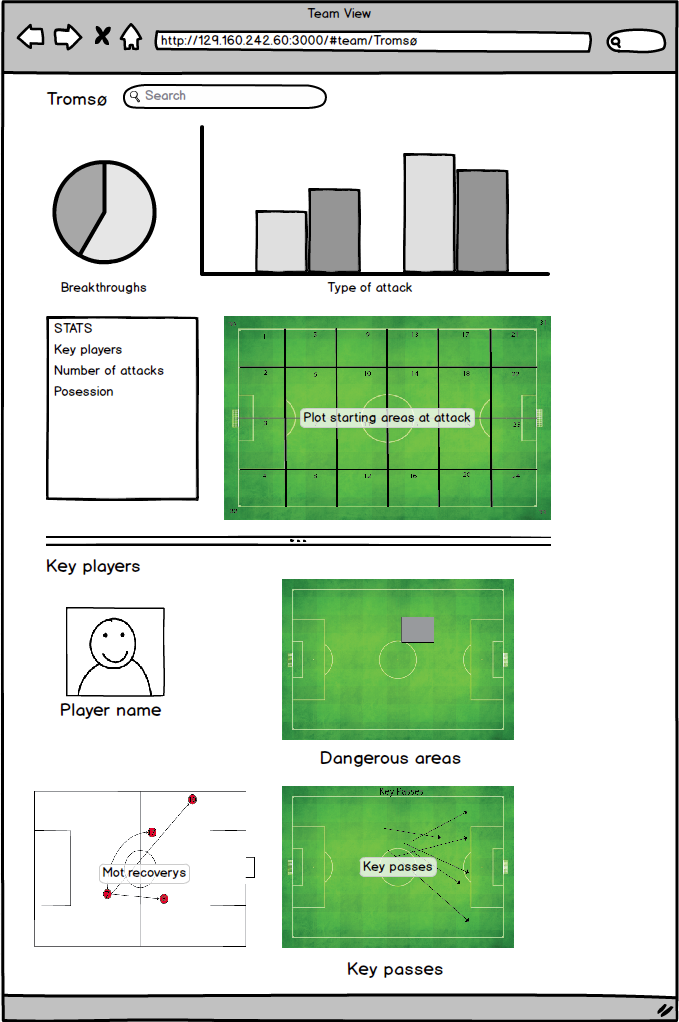
\includegraphics[width=150mm]{images/general/mockup.png}
\caption{All matches registrated in the database are listed on this page}
\label{overflow}
\end{figure}


\subsection{}

The first page you are prompted with is the listing of all matches registered in the database. A click on match gives you details about that match and prompts you a interface for capturing new attacks if requested. Every field has to be submitted with an correct input value.

\begin{figure}[ht!]
\centering
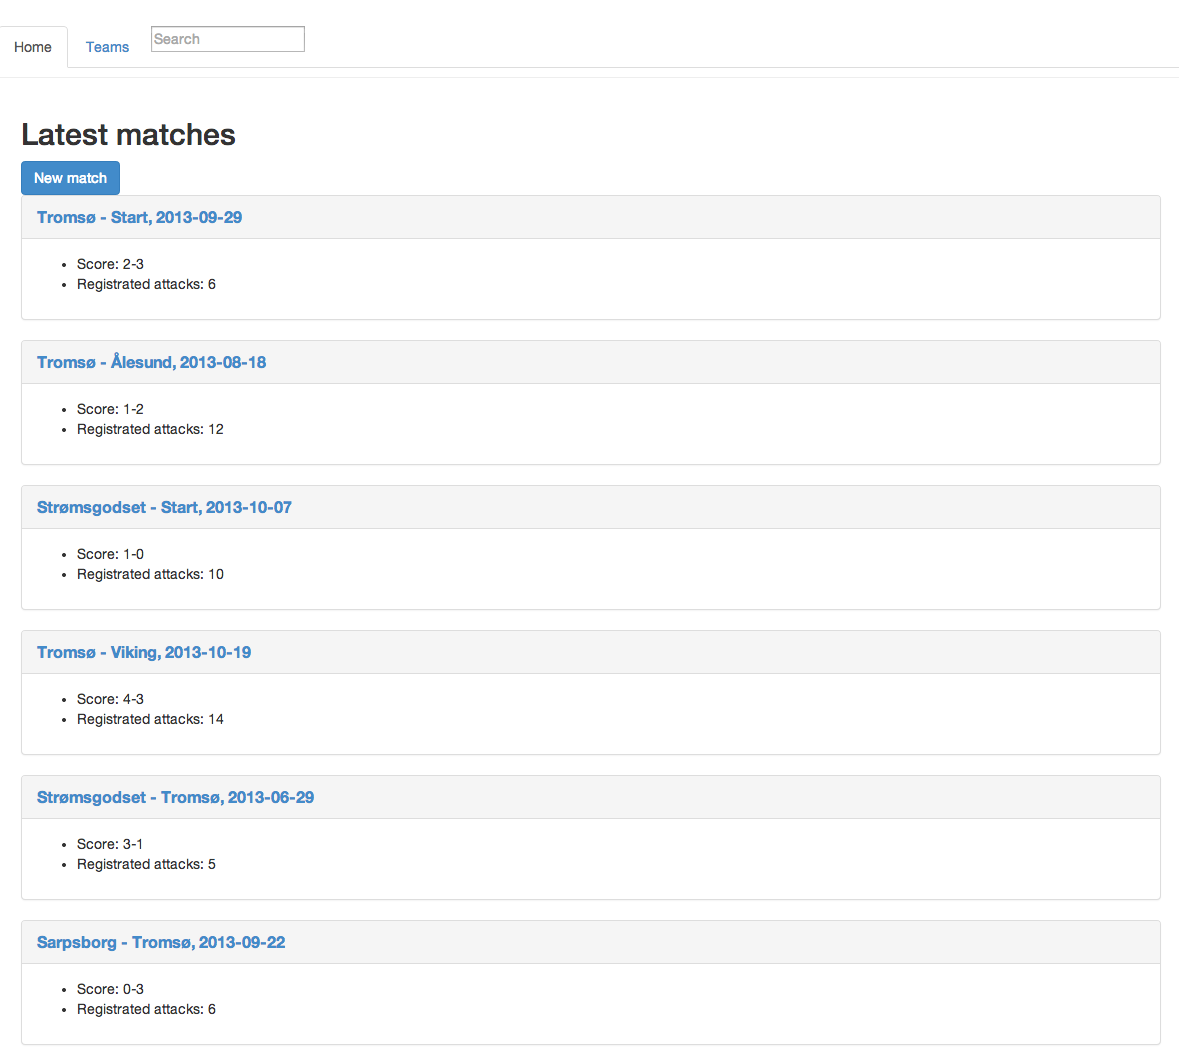
\includegraphics[width=100mm]{images/general/all_matches.png}
\caption{All matches registrated in the database are listed on this page}
\label{overflow}
\end{figure}


